\documentclass{article}
\usepackage{amsmath, amssymb, graphicx, subfigure, algorithmic, color}

\author{Mitchell Koch, Justin Huang}
\title{Learning Relation Entailment Graphs\\CSE 515 Final Report}
\date{Friday, June 14, 2013}

\begin{document}
\maketitle

\begin{abstract}
Can learning relation entailment graphs based on WordNet or Bayes net
structure learning improve relation query performance?
\end{abstract}

\section{Introduction and Motivation}

Open IE~\cite{Etzioni:2008:OIE:1409360.1409378}

previous relation entailment
work~\cite{Berant:2012:LER:2122944.2122947, berant2011global}, on work in relation
extraction using matrix factorization~\cite{riedel13relation}, 

as well as on related work in probabilistic modeling of relations
between entities~\cite{TaskarWAK03, Taskar:2002:DPM:2073876.2073934}.

Freebase using distant supervision as in~\cite{HoffmannZLZW11}

\subsection{Database Query Task}
\label{database-query-task}
We define the following database query task to evaluate a relation entailment graph. Let $R$ be a set of relation strings, and $A$ be a set of argument strings. We are given a database $D$ of facts, where each fact is of the form $r(x, y)$ for some $r\in R$ and $x, y\in A$.

Given a query for a relation $r$ with arguments $x$ and $y$, we can expand the query to additionally search for all $r^\prime(x, y)$ such that there exists an edge from $r^\prime$ to $r$ in the entailment graph. An example of this process is shown in Figure~\ref{query-expansion}. We can then evaluate the correctness of the returned results.

\begin{figure}[h]
\begin{center}
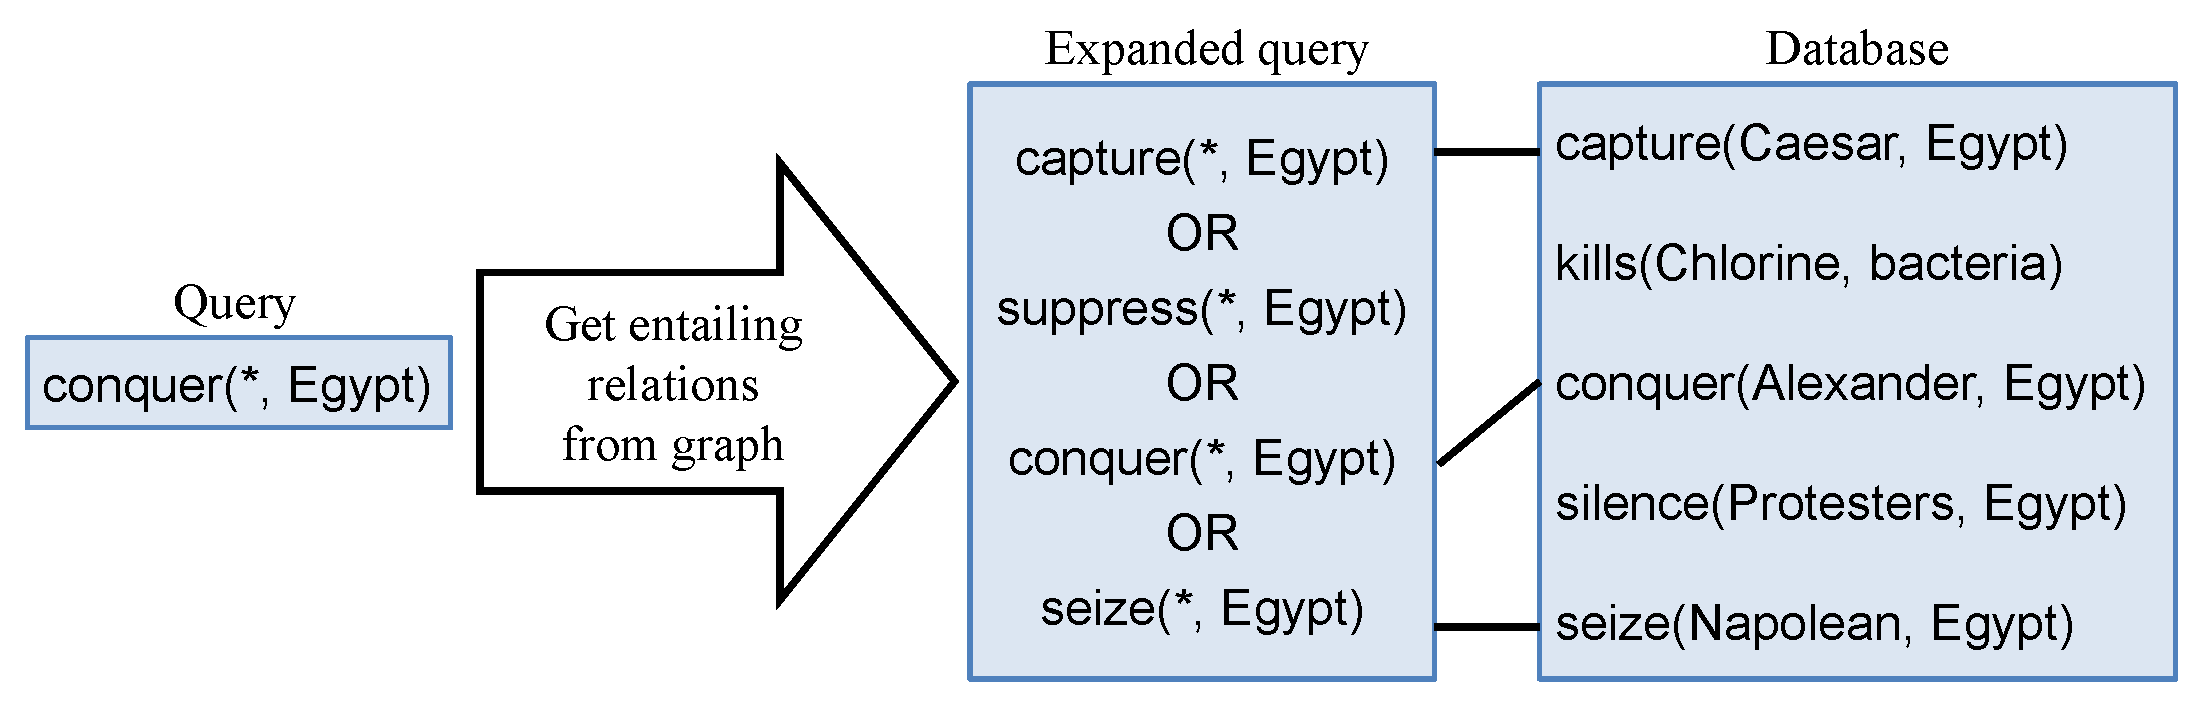
\includegraphics[width=1.0\textwidth]{figures/query-expansion.pdf}
\end{center}
\caption{An example of a query being expanded.}\label{query-expansion}
\end{figure}

\section{Methods and Algorithms}

\subsection{Constraints on WordNet}

WordNet~\cite{fellbaum98wordnet} is a hand-crafted resource that distinguishes between different word senses, and provides synonyms and entailments between them. We denote a WordNet sense with a number where \textit{\#1} is the most common. For example \textit{note\#4} is the fourth most common sense of ``note,'' which means ``to write down''. Each WordNet sense has its sense number, a count indicating how often that sense is used, and a probability, which is the count divided by the sum of counts for all senses of the same word.

\subsubsection{WordNet entailment graph}
A troponym is a specialization of a word, e.g., ``to fly'' is a troponym of ``to travel.'' We say that WordNet sense $w_1$ entails $w_2$ if $w_1$ is a synonym of $w_2$, if $w_1$ is a troponym of $w_2$ in WordNet, or if there exists some $w_3$ such that $w_1$ entails $w_3$ and $w_3$ entails $w_2$. A path in the entailment graph is defined as the sequence of troponyms between $w_1$ and $w_2$. The entailment graph is disconnected. Figure ~\ref{wordnet-graph} shows one component of the graph, and Figure ~\ref{example-path} shows an example of a path in the graph, from \textit{note\#4} to \textit{write\#2}.

\begin{figure}[h]
\begin{center}
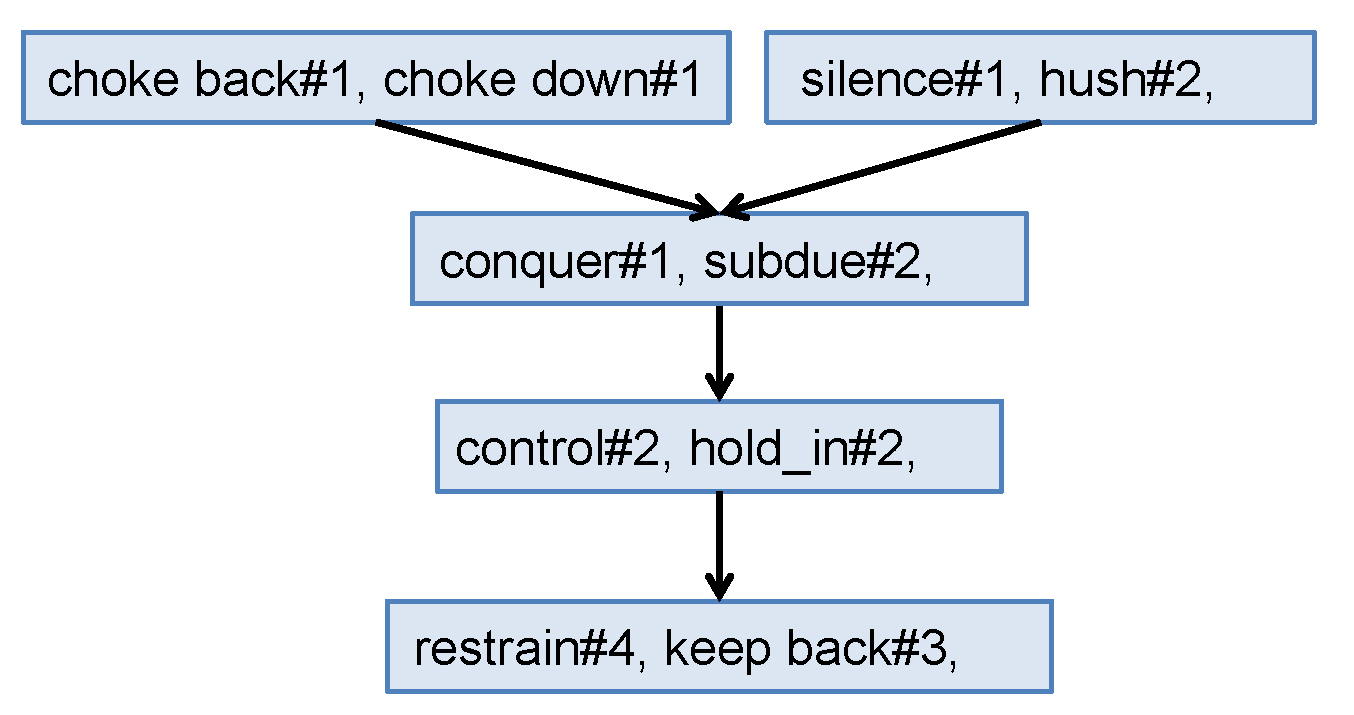
\includegraphics[width=0.6\textwidth]{figures/wordnet-graph.pdf}
\end{center}
\caption{Component of the WordNet entailment graph with the first sense of conquer, \textit{conquer\#1}. Boxes represent synonym sets, arrows represent entailments.}\label{wordnet-graph}
\end{figure}

\begin{figure}[h]
\begin{center}
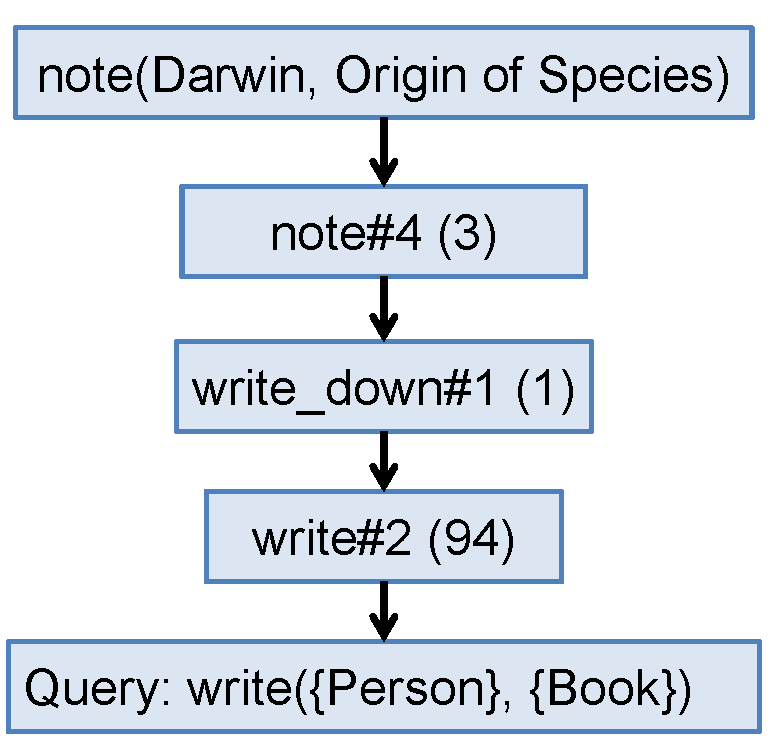
\includegraphics[width=0.4\textwidth]{figures/example-path.pdf}
\end{center}
\caption{Example path in entailment graph}\label{example-path}
\end{figure}

Although WordNet already defines an entailment graph between verb senses, one hurdle to using it is determining what sense to use. For example, given the verb ``take,'' is it \textit{take\#21} (take by force) or \textit{take\#2} (take time)? Each sense will lead to very different entailments. The first part of our approach is to assume a string can take on any of its WordNet senses, which may lead to noisier entailments. The second part is to train a logistic regression classifier to help filter out noisy entailments.

\subsubsection{Logistic regression classifier}
For a certain set of queries, we use all possible entailments from WordNet on the database query task, and label each fact as relevant to the query or not relevant to the query. This data is subsequently used to train the logistic regression model. For each result, we record the path that was taken in the entailment graph and produce the following features:
\begin{enumerate}
  \item Path length
  \item Average sense number
  \item Average WordNet probability
  \item Maximum sense number
  \item Minimum WordNet probability
\end{enumerate}

The length of the path is how many nodes there were in the path. For example, in figure ~\ref{example-path}, the length is 3. Because WordNet senses are ranked in order frequency, we use the average and maximum sense numbers as features, the idea being that an uncommon WordNet sense (e.g., \textit{take\#42}) could be a weak link in the entailment path. A similar intuition holds for the probabilities of the WordNet senses.

The output of logistic regression is a set of weights $w$ for each feature. Let $x$ be the vector of features described above. Then the probability of the label we would like to predict is given by:
\begin{align*}
  p(x) = \frac{e^{w\cdot x}}{1 + e^{w\cdot x}}
\end{align*} 

\subsection{Bayesian Network Structure Learning}

\begin{figure}[h]
\begin{center}
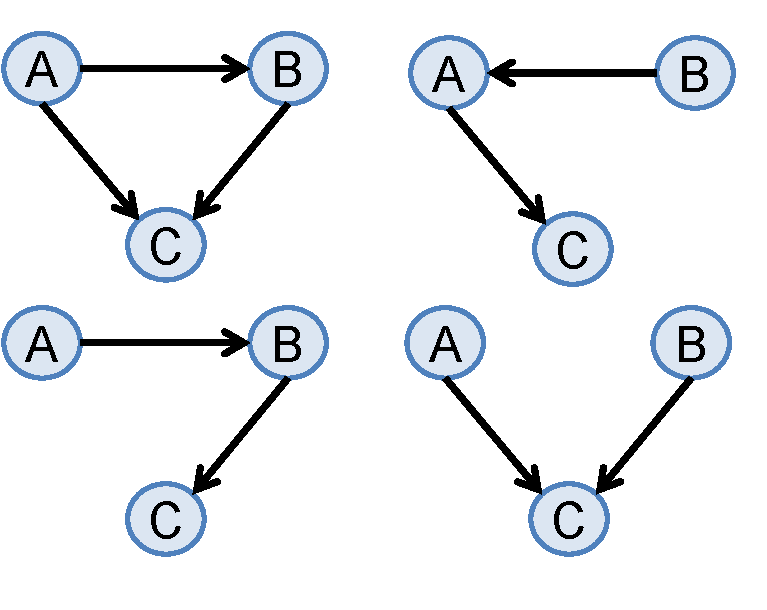
\includegraphics[width=0.4\textwidth]{figures/example-net-structures.pdf}
\end{center}
\caption{Examples of possible network structures}\label{example-net-structures}
\end{figure}


\section{Experiments and Results}
We evaluated our relation entailment graphs on the database query task, as described in section ~\ref{database-query-task}. The set of queries we chose to evaluate with are listed in table ~\ref{benchmark-queries}.

\begin{figure}[h]
  \begin{center}
    \begin{tabular}{ | l | }
      \hline
      Query\\
      \hline
      has-written(type: Person, type: Book)\\
      play(Tom Hanks, ?)\\
      conquer(?, Egypt)\\
      killed(?, Voldemort)\\
      grown-in(coffee, type: Country)\\
      \hline
    \end{tabular}
  \end{center}
  \caption{Benchmark queries for database query task.}\label{benchmark-queries}
\end{figure}

Our baseline is a system that does no query expansion, only searching the database for an exact string match of the relation phrase. We compared this to systems that expanded queries based on the entailment graphs from 1) all of WordNet, 2) WordNet with logistic regression, and 3) Bayes net structure learning.

We labeled the results from the full WordNet system, and trained the logistic regression model on the labeled data using 10-fold cross validation.

The input to the structure learning was a matrix of counts, with relation phrases for rows and entity pairs for columns. However, we were constrained by high memory usage when running structure learning on graphs with more than 150 relation phrases. As a result, for some queries, we had to randomly sample 150 relation phrases. The search was done using 100 samples of Markov Chain Monte Carlo (MCMC), with a burn-in of 10.

Our results are summarized in figure ~\ref{results}. Structure learning had no effect on the results because none of the entailments learned through structure learning applied to the five queries listed in figure ~\ref{benchmark-queries}.

\begin{figure}[h]
  \begin{center}
    \begin{tabular}{ | l | l | l | }
      \hline
      System & \# results returned & Precision\\
      \hline
      Baseline & 115 & 83.48\%\\
      Structure learning & 115 & 83.48\%\\
      WordNet & 1105 & 86.85\% \\
      WordNet + logistic regression & 1035 & 91.50\%\\
      \hline
    \end{tabular}
  \end{center}
  \caption{Results on database query task for queries in figure ~\ref{benchmark-queries}.}\label{results}
\end{figure}

These results show that using entailments from WordNet improved recall substantially. We were surprised that using WordNet entailments also increased precision, but that likely stems from our choice of queries. For example, while not many facts in the database specifically say a person ``has written'' a book, many facts say a person ``writes'' a book. Since we consider those to be correct answers, those results push precision up. Adding the logistic regression classifier presented us with a precision/yield tradeoff.

To see the results of structure learning, we also tried a set of 10 benchmark queries that had entries in the entailment graph generated from structure learning. The queries are listed in figure ~\ref{structure-queries}, and our results are shown in figure ~\ref{structure-results}.

\begin{figure}[h]
  \begin{center}
    \begin{tabular}{ | l | l | l | }
      \hline
      System & \# results returned & Precision\\
      \hline
      Baseline & 55 & 98.18\%\\
      Structure learning & 73 & 76.71\%\\
      WordNet & 108 & 56.48\% \\
      WordNet + logistic regression & 58 & 91.38\%\\
      \hline
    \end{tabular}
  \end{center}
  \caption{Results on database query task for queries in figure ~\ref{structure-queries}.}\label{structure-results}
\end{figure}

This set of results shows that structure learning will increase the number of results returned, but at a high cost to precision. These results also show that for the type of more specific queries presented in ~\ref{structure-queries}, almost all the extra results given by WordNet entailments are bad. The classifier partially recovered the loss in precision.

\begin{figure}[h]
  \begin{center}
    \begin{tabular}{ | l | }
      \hline
      Query\\
      \hline
      be-one-of(coffee, type:Country)\\
      work-on(type:Person, type:Book)\\
      be-solidly-establish in(coffee, type:Country)\\
      believe-in(type:Person, type:Book)\\
      play-major-economic-role-in(coffee, type:Country)\\
      be-come-in(type:Person, type:Book)\\
      discuss-character-of(Tom Hanks, ?)\\
      be-originally-find-in(coffee, type:Country)\\
      tell(Tom Hanks, ?)\\
      endorse(Tom Hanks, ?)\\
      \hline
    \end{tabular}
  \end{center}
  \caption{Benchmark queries to evaluate structure learning.}\label{structure-queries}
\end{figure}

\section{Discussion and Conclusion}
Our results suggest that the choice of benchmark queries can make a big difference in the results. However, we noticed that using WordNet with a classifier does seem to increase yield at an acceptable level of precision. Although it's hard to say what queries should be used in our experiment, the queries in figure ~\ref{benchmark-queries} are arguably more common than those in figure ~\ref{structure-queries}.

% Issues with structure learning (edge direction, scalability, etc.)

\bibliographystyle{abbrv}
\bibliography{bib}

\end{document}
